\subsection{Other learners and alarm settings}\label{sec:res-robust}

The fourth amendment repeated the validity analysis (repetition~0, same units and splits) with three further learners, ridge regression and a random forest on the causal features and a multilayer perceptron on the raw normalised sensors of the last 30 rows, and with 27 settings of the GBM signal (cap, smoothing span and debounce, three values each). The GBM reference reproduced the main run's decisions exactly on all seven datasets. With every learner the conformal notice alarm kept its level (Fig.~\ref{fig:robust}a): at $\alpha=0.10$ and the primary lead time the three new learners failed on 4.0--17.0\,\% of test units on individual datasets and on 9.3--9.9\,\% pooled over datasets, and no exact test exceeded 10\,\% after Holm's correction (smallest adjusted $p=0.43$; H11 supported). Pooled over datasets and lead times, all four learners gave 3.9--4.2, 9.5--10.0 and 18.5--19.6\,\% at nominal 5, 10 and 20\,\%. The per-cycle lower bound calibrated over all rows failed on 20--70\,\% of units with the random forest and 26--71\,\% with ridge regression, significantly above 10\,\% on all seven datasets, and on 6--38\,\% with the perceptron, significantly on five (H12 supported). Restricting its residuals to rows near failure, which nearly repaired it for GBM, did not repair it for ridge regression (17--33\,\%) and only partly for the random forest (up to 17\,\%): how well that repair works depends on the learner as well as on the choice of rows. A weaker signal cost CNA notice rather than reliability: with ridge regression the median notice at the primary lead time was 18--21 cycles on PHM08 and C-MAPSS against 15.5--16 with GBM (on N-CMAPSS 23 against 25), and with the perceptron 64 battery cycles against 42. Across the 27 settings of the GBM signal the pooled failure rate stayed between 8.7 and 11.1\,\% (H13 supported) and the mean notice between 17.4 and 18.1 engine cycles (battery 41--48): once the critical level is calibrated, the a-priori choice of these settings hardly matters for either.

\begin{figure*}[t]\centering
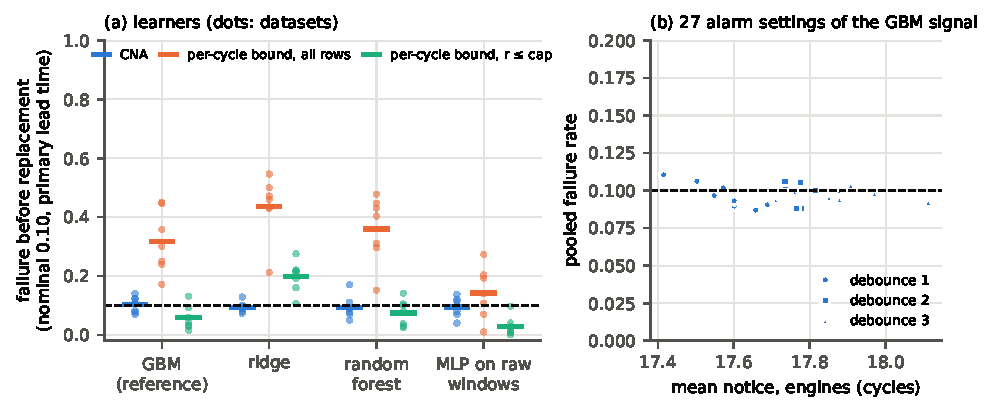
\includegraphics[width=0.95\textwidth]{figures/Fig8_robustness.pdf}
\caption{Other learners and alarm settings (repetition~0, primary lead time). (a) Failure before replacement at nominal 0.10 for CNA and the per-cycle lower-bound alarms built on four learners fitted to the same units; dots: datasets, bars: their mean. (b) Pooled failure rate of CNA at $\alpha=0.10$ against the mean notice on the engine datasets for 27 settings of the GBM signal (cap $\times$ smoothing span $\times$ debounce).}\label{fig:robust}
\end{figure*}
